\section{Background}

\note[Luca][notesyellow]{Introduction to HEP community, with mention to WLCG as an essential tool to perform their research}

% High-Energy Physics (HEP) is a branch of physics that studies the fundamental constituents of matter and the forces that drive their interactions. One of the methods is to create very high energy densities. 
% This reproduces the environmental conditions of the primordial universe.

High-Energy Physics (HEP) is a branch of physics that studies the elementary constituents of matter and the fundamental principles that govern their interaction to understand how our universe formed and evolved.  
These particles, however, are not visible at the scales whereby we experience reality today. 
Thus, HEP experiments need to either look at natural phenomena generated in pressure and temperature conditions similar to those in the primordial universe -- like cosmic rays -- or recreate such settings artificially.

The European Council for Nuclear Research (CERN) laboratory is part of this second strand of experiments, and it constitutes the largest particle physics laboratory in the world.
From 2008, CERN facilities also include the Large Hadron Collider (LHC), the longest particle accelerator ever built.
LHC consists of a 26.7-kilometer ring located in a tunnel about 100 meters underground in the Geneva area, and it is made of superconducting magnets with several accelerating structures.
Inside the accelerator, bunches of protons are revved up to nearly the speed of light, forming two high-energy particle beams that travel in opposite directions inside separated pipes. 
When they acquire the desired energy, the beams are directed towards dedicated interaction points where the experiments occur.%surrounded by giant detectors.
In practice, LHC hosts four major experiments -- ATLAS, ALICE, LHCb and CMS -- built in correspondence of these interaction points and equipped with giant detectors.
Once the beams get there, the two pipes cross and the particles are squeezed through substantial magnetic fields to increase their chances of colliding. 
In this way, a massive amount of energy is concentrated in an extremely tiny area, generating millions of particles at each collision.

Although not the most popular among the mainstream audience, the HEP community is one of the most prominent players concerning big data.
In fact, the high speed of the beams causes roughly 40 million crossings per second at each interaction point. 
When a crossing happens, an average of 15 bunch collisions are observed  (also referred to as pileup). The particles produced by each scattering then fly around the interaction point to be eventually detected through high-technology experimental devices endowed with 100 million signal channels.
According to the current experimental setup, this delivers 100 MegaBytes (MB) of data per collision and it would generate 40k ExaBytes (EB) every year.
However, acquiring and storing such a tremendous amount of data is unattainable with current technology/budget. In addition, the events of interest are typically rare, so there is actually no need to store all of that information.
Thus, the vast majority of data from collisions is discarded straight away and the event rate is lowered to 1k crossings per second. 
As a result of this reduction, the actual acquisition rate amounts to 1MB every second, translating to roughly 100 PetaBytes (PB) a year in 2020.
Besides that, physics analyses require comparing experimental results with simulated data according to current theories, thus producing somewhat between 1 and 2 times additional data.
Furthermore, the CERN collaboration is already working at enhancing the Large Hadron Collider capabilities.
The project involves boosting the energy of the beam and gradually increasing the pileup towards 150 collisions per bunch crossing.
Thanks to this upgrade, way more events will be observed as the beam energy will be boosted and the pileup will gradually be increased towards 150 collisions per bunch crossing.
In this new regime, an estimated 400 PB of new data will be generated each year by 2026, thus leading to the so-called High Luminosity LHC (HL-LHC).

\note[Luca][notesyellow]{Introduction to grid/distributed computing/WLCG}


\subsection{The Worldwide LHC Computing Grid}

\sidenote[Luca][notesyellow]{Cos'è WLCG?}
The Worldwide LHC Computing Grid (WLCG) is a global computing infrastructure whose mission is to provide computing resources to store, distribute and analyse the data generated by the Large Hadron Collider (LHC), making the data equally available to all partners, regardless of their physical location.

WLCG is the world's largest computing grid. It is supported by many associated national and international grids across the world, such as European Grid Initiative (Europe-based) and Open Science Grid (US-based), as well as many other regional grids.

WLCG is co-ordinated by CERN. It is managed and operated by a worldwide collaboration between the experiments (ALICE, ATLAS, CMS and LHCb) and the participating computer centres. It is reviewed by a board of delegates from partner country funding agencies, and scientifically reviewed by the LHC Experiments Committee.

\sidenote[Luca][notesyellow]{Cosa fa WLCG?}
WLCG provides seamless access to computing resources which include data storage capacity, processing power, sensors, visualization tools and more. Users make job requests from one of the many entry points into the system. A job will entail the processing of a requested set of data, using software provided by the experiments

The computing Grid establishes the identity of the user, checks their credentials, and searches for available sites that can provide the resources requested. Users do not have to worry about where the computing resources are coming from – they can tap into the Grid's computing power and access storage on demand.


\sidenote[Luca][notesyellow]{WLCG community}
The Worldwide LHC Computing Grid (WLCG) is a distributed computing infrastructure arranged in tiers – giving a community of over 12,000 physicists near real-time access to LHC data. Data pours out of the LHC detectors at a blistering rate. Even after filtering out 99\% of it, in 2018 we gathered 88 petabytes of data. That's 88 million gigabytes, the equivalent to around 22 million high-definition (HD) movies.

\sidenote[Luca][notesyellow]{Cos'è WLCG?}
The scale and complexity of data from the LHC is unprecedented. This data needs to be stored, easily retrieved and analysed by physicists all over the world. This requires massive storage facilities, global networking, immense computing power, and, of course, funding.

\sidenote[Luca][notesyellow]{Inserire qui una descrizione dell'infrastruttura}

\sidenote[Luca][notesyellow]{Ordini di grandezza}
The next LHC Run is scheduled for 2021-2023. This looks to be even more challenging than the previous runs; data archiving is expected to be double what it was for LHC Run 2, and Run 4 - in HL-LHC operation - is even expected to be fives times that. 

The requirements for data and computing will grow dramatically during this time, with rates of 500 PB/year expected for the HL-LHC. The needs for processing are expected to increase more than 10 times over and above what technology evolution will provide. As a consequence, partnerships such as those with CERN openlab and other programmes of research and development are essential to investigate how the computing models could evolve to address these needs. They will focus on applying more intelligence into filtering and selecting data as early as possible. Investigating the distributed infrastructure itself (the grid) and how one can best make use of available technologies and opportunistic resources (grid, cloud, HPC, volunteer, etc), improving software performance to optimise the overall system.








$$\dots$$

% One of the biggest collaborations working on distributed computing is the WLCG. 
% The LHC grid has a very layered topology, both in terms of physical organization and of ...
% is made of many services, each taking care of specific sub-processes that together enables the global functioning of the whole infrastructure.
\sidenote[Luca][notesyellow]{Explain why data are moved around by these communities}
In such a vast environment, a great deal of attention is devoted to the data, which are arguably the most valuable good of the community.
For example, specific distribution and redundancy policies have been set to prevent data loss. Also, a careful design is put in place to guarantee a FAIR access to them.
In particular, data must be available at any time for researchers to analyse them and contribute to the progression of science in their sectors.
\sidenote[Luca][notesyellow]{introduce transfer failures}
Consequently, massive amounts of data -- both in size and number -- are frequently moved across the grid, occasionally experiencing failures ranging from a user mistyping a command to more severe software/hardware defects that require prompt intervention. 
For this reason, data transfer processes are continuously monitored by teams of shifters whose job is to detect issues and report them to experts that take care of their solution.
\lc{Here goes some reference to the orders of magnitude at stake, i.e.: 
\begin{itemize}
    \item n. tranfers/day (whole or per virtual organization) --> can retrieve from FTS
    \item ticket/year or month or day (whole or per virtual organization) --> how to retrieve that? is there any official source?
\end{itemize}
}

Due to the complexity of the infrastructure and its layered structure, identifying potential problems, understanding their causes and fixing them may take a while, thus demanding a great human effort.
\lc{Describe current operations and possibly volumes: 
\begin{itemize}
    \item Current operations: efficiency matrix + drill down (description + falls)
    \item average solving time $\rightarrow$ how to retrieve that? is there any official source?
    \item n. people involved (both shifters and sites) $\rightarrow$ how to retrieve that? is there any official source?
\end{itemize}
}
%Current operations are based on a site-centric monitoring approach that involves mainly manual, post-mortem reporting. In this approach, trained operators look at Grafana dashboards that act as a high-level overview of the systems status and try to spot hints of incorrect or undesired behaviours.
Current operations are based on a site-centric approach where trained personnel monitor the status of the various services almost 24/7 and try to spot hints of incorrect or undesired behaviours. In particular, they look at Grafana dashboards acting as a high-level overview of the system. A usual starting point is the so-called efficiency matrix (Figure \ref{fig:efficiency_matrix}), where the percentage of successful transfers is reported at customisable levels ranging from cloud to site, endpoint or even space token.
\begin{figure}
    \centering
    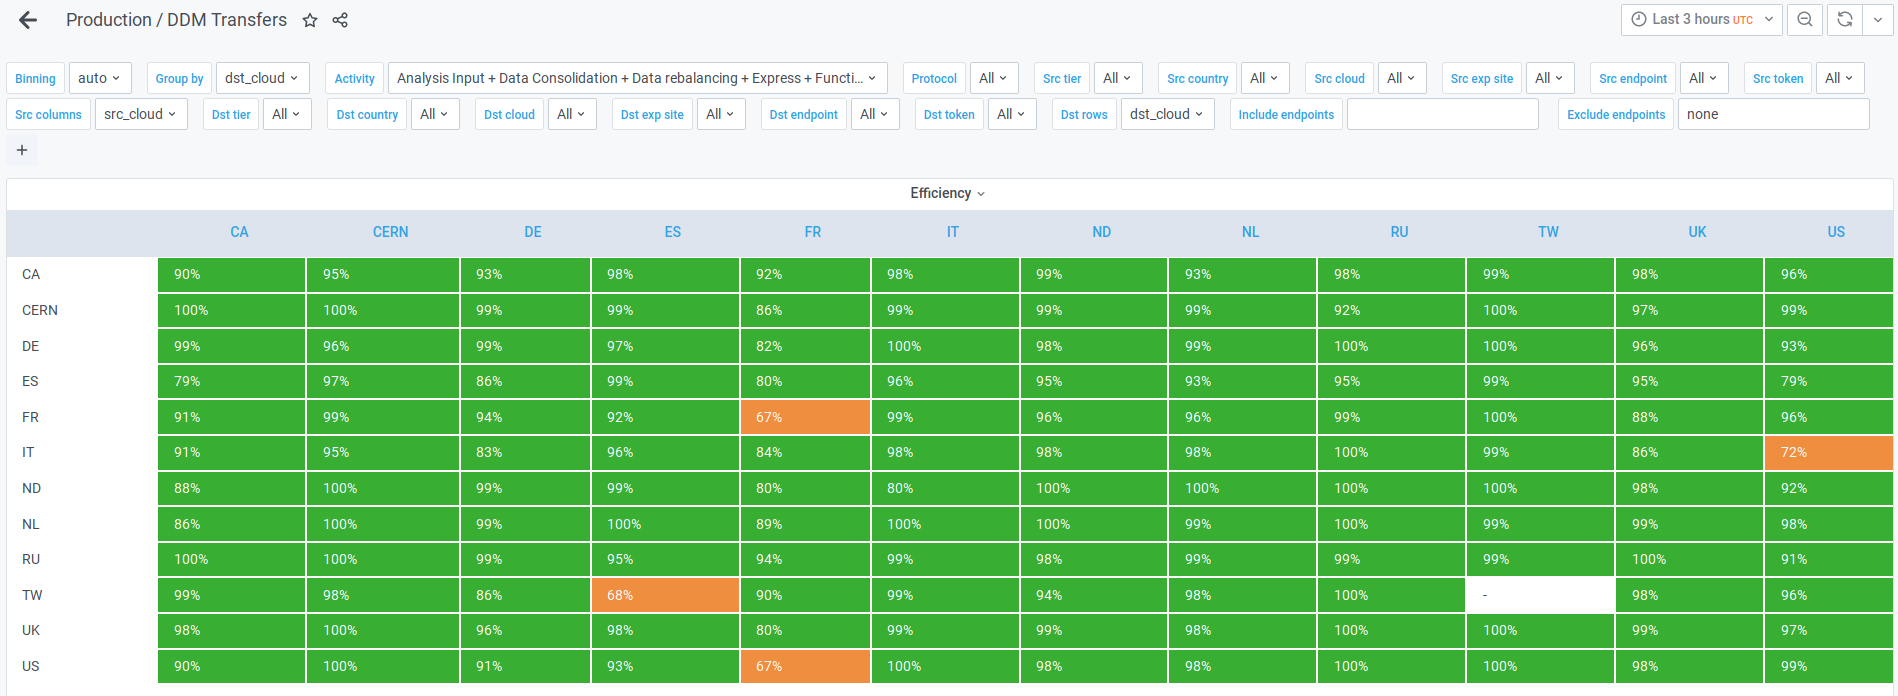
\includegraphics[width=\textwidth]{figures/220_introduction/efficiency_matrix.png}
    \caption{Transfer efficiency matrix from Grafana. Transfer sources are shown as columns and destinations as row. The drop-down menus at the top allow custom filtering.}
    \label{fig:efficiency_matrix}
\end{figure}
When the efficiency falls below an acceptable threshold, typically 60-70\%, on-duty shifters start to investigate the issue at a lower level by checking \emph{i)} where the error happened, \emph{ii)} how many errors are produced, \emph{iii)} what is the time pattern (temporary, extended or cyclical) and \emph{iv)} which error messages are generated. 
However, this procedure gives rise to many false alarms as it is usual to encounter problems that do not represent a real concern. This typically happens when the failure rate is high because just a few transfers were attempted, or there was a transient issue that was already fixed. 
Also, sometimes unnecessary drill-down activity is performed for actual issues that were already known, as in the case of ongoing tickets or site downtimes, for which reporting is not required.
As a result, many human resources are employed in repetitive tasks of little scientific interest that would enormously benefit from automation. 

\sidenote[Luca][notesyellow]{Describe also why a site-centric approach is not optimal and how a message-centric one could help}
In addition to that, a site-centric strategy as described above has some drawbacks. Firstly, monitoring focuses on spotting where issues occur, while understanding the actual root causes is typically demanded to site experts in a subsequent investigation.
Secondly, problems generating few error messages are usually ignored. This is natural, and to some extent desirable, as having limited resources forces us to address bigger misfunctioning first. However, that could be a potential pitfall in cases where promptly fixing a minor issue may prevent the rising of a more significant and longer to solve defect.

All these problems could be tackled programmatically by standardising the logging output of all the services. In this way, neat error messages would point directly to the source of the problem, thus allowing complete automation. 
However, the distributed nature of the infrastructure hampers such an approach.
In fact, the opportunistic gathering of computing resources that led to WLCG entails many local configurations that are not easy to address using only a static strategy.
Hence, all these considerations expose the need for an intelligent support tool for speeding up infrastructure management to meet the productivity requirements for the near future.

% Hence, the current approach will no longer meet the productivity requirements in the near future given the limited resources

\subsection{Contribution}
The goal of this work is to discuss a complementary, experiment-agnostic, computer-aided approach to grid monitoring centered on error messages rather than site performances.

In particular, we propose an unsupervised Machine Learning (ML) pipeline to identify clusters of similar failures. These groups are then exposed to shifters as suggestions of potential issues to investigate further.